% 第 19 章 Extending the Graphical User Interface
\bichapter{扩展图形用户界面}{Extending the Graphical User Interface}
\label{chap:gui-ext}

IC Compiler II 图形用户界面（GUI）提供一套丰富的应用程序编程接口（application programming interface，API），用于定制菜单、按钮以及 GUI 的其他元素。可用该 API 创建自定义按钮、菜单项（menu item）和地图模式（map mode），并把它们关联到工具中的自定义函数或内建函数。定制可以在工具启动时自动加载，也可以稍后通过 source 脚本文件中的命令来添加。

此外，工具支持标注（annotation）。可用标注在版图视图（layout view）上绘制直线、矩形、多边形、符号和文字。

下列主题说明不同类型的 GUI 定制：
\begin{itemize}
  \item 创建菜单项
  \item 向 Favorites 调色板添加按钮
  \item 用 Tcl 命令高亮对象
  \item 创建标注
  \item 保存标注
  \item 创建新的视觉模式
\end{itemize}

% ============================================================
\section{创建菜单项}
\subsection*{Creating Menu Items}

IC Compiler II 工具通过 \cmd{gui\_create\_menu} 及其他命令支持菜单定制。使用 \cmd{gui\_create\_menu} 命令修改菜单栏（menu bar）并添加新命令；使用 \cmd{gui\_set\_hotkey} 命令定义或重新定义热键（hotkey）。

下列彼此独立的示例逐步增加菜单定制的复杂度，用于建立名为 \textbf{Nudge Left} 与 \textbf{Nudge Right} 的新菜单项。这两项分别把视图略微向左、向右平移（pan）。

\begin{itemize}
  \item 定义两个基本菜单项，见图~\ref{fig:gui-193}。
\end{itemize}

\begin{figure}[htbp]
\centering
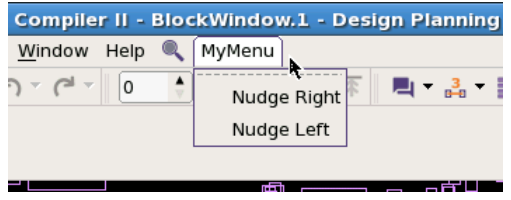
\includegraphics[width=0.92\textwidth]{gui-fig-193.png}
\caption{简单菜单项}
\label{fig:gui-193}
\end{figure}

\begin{lstlisting}
gui_create_menu -menu "MyMenu->Nudge Right" \
   -tcl_cmd {gui_scroll \
   -window [gui_get_current_window -view] -hrel .05}

gui_create_menu -menu "MyMenu->Nudge Left" \
   -tcl_cmd {gui_scroll \
   -window [gui_get_current_window -view] -hrel -.05}
\end{lstlisting}

\begin{itemize}
  \item 在上一例的基础上，为这些菜单项创建标题（heading），并插入一条分隔线（separator），见图~\ref{fig:gui-194}。
\end{itemize}

\begin{figure}[htbp]
\centering
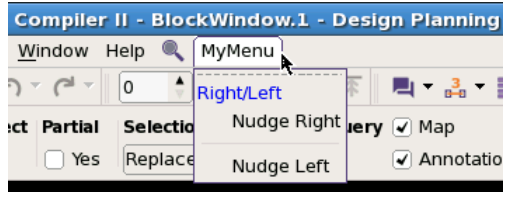
\includegraphics[width=0.92\textwidth]{gui-fig-194.png}
\caption{带标题与分隔线的菜单}
\label{fig:gui-194}
\end{figure}

\begin{lstlisting}
gui_create_menu -menu "MyMenu->Right/Left" -heading "Right/Left"
gui_create_menu -menu "MyMenu->Nudge Right" \
   -tcl_cmd {gui_scroll \
      -window [gui_get_current_window -view] -hrel .05}

gui_create_menu -menu "MyMenu->___" -separator
gui_create_menu -menu "MyMenu->Nudge Left" \
   -tcl_cmd {gui_scroll \
      -window [gui_get_current_window -view] -hrel -.05}
\end{lstlisting}

\begin{itemize}
  \item 在上一例的基础上，把新菜单项放在 \textbf{Help} 菜单左侧一个位置，并为每个菜单项定义自定义图标，见图~\ref{fig:gui-195}。
\end{itemize}

\begin{figure}[htbp]
\centering
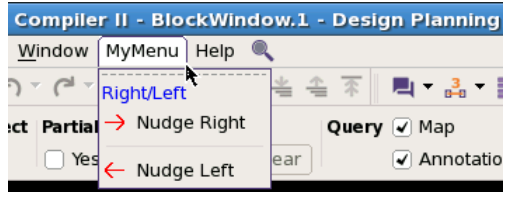
\includegraphics[width=0.92\textwidth]{gui-fig-195.png}
\caption{指定位置的菜单}
\label{fig:gui-195}
\end{figure}

\begin{lstlisting}
gui_create_menu -menu "MyMenu->Right/Left" \
   -heading "Right/Left" \
   -anchor_item Help \
   -anchor_offset -1
gui_create_menu -menu "MyMenu->Nudge Right" \
   -tcl_cmd {gui_scroll \
   -window [gui_get_current_window -view] -hrel .05} \
   -icon_file /u/user/icons/right_16_xpm.xpm
gui_create_menu -menu "MyMenu->___" -separator
gui_create_menu -menu "MyMenu->Nudge Left" \
   -tcl_cmd {gui_scroll \
   -window [gui_get_current_window -view] -hrel -.05} \
   -icon_file /u/user/icons/left_16_xpm.xpm
\end{lstlisting}

\begin{itemize}
  \item 在上一例的基础上，先用 \cmd{gui\_create\_menu} 命令定义菜单项，再用 \cmd{gui\_set\_hotkey} 命令重新定义热键。热键定义会显示在菜单中，见图~\ref{fig:gui-196}。
\end{itemize}

\begin{figure}[htbp]
\centering
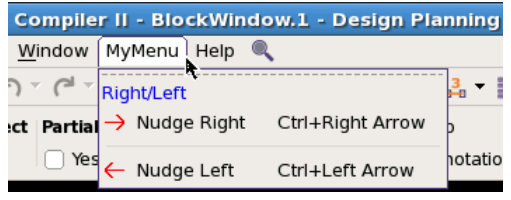
\includegraphics[width=0.92\textwidth]{gui-fig-196.png}
\caption{带热键定义的菜单}
\label{fig:gui-196}
\end{figure}

\begin{lstlisting}
gui_set_hotkey -replace -hot_key Ctrl+Right \
   -menu "MyMenu->Nudge Right"
gui_set_hotkey -replace -hot_key Ctrl+Left \
   -menu "MyMenu->Nudge Left"
\end{lstlisting}

如果热键此前尚未分配，可以用 \cmd{gui\_create\_menu} 命令的 \opt{-hot\_key} 选项来分配。本例使用 \cmd{gui\_set\_hotkey} \opt{-replace} 覆盖已有的热键设置。

% ============================================================
\section{向 Favorites 调色板添加按钮}
\subsection*{Adding Buttons to the Favorites Palette}

可以把按钮添加到收藏夹调色板（Favorites palette）。这是新建工具栏（toolbar）之外的另一种做法。要把一个按钮项加到 Favorites 调色板：
\begin{enumerate}
  \item 按 F10 打开 Favorites 调色板。
  \item 单击某个按钮，并将其拖到 Favorites 调色板上。
\end{enumerate}

要用命令搜索（command search）找到按钮项并加到 Favorites 调色板：
\begin{enumerate}
  \item 按 F10 打开 Favorites 调色板。
  \item 单击放大镜，打开命令搜索。
  \item 输入命令或任务名称。
  \item 在结果列表中单击该项，并将其拖到 Favorites 调色板上。
\end{enumerate}

见图~\ref{fig:gui-197}。

\begin{figure}[htbp]
\centering
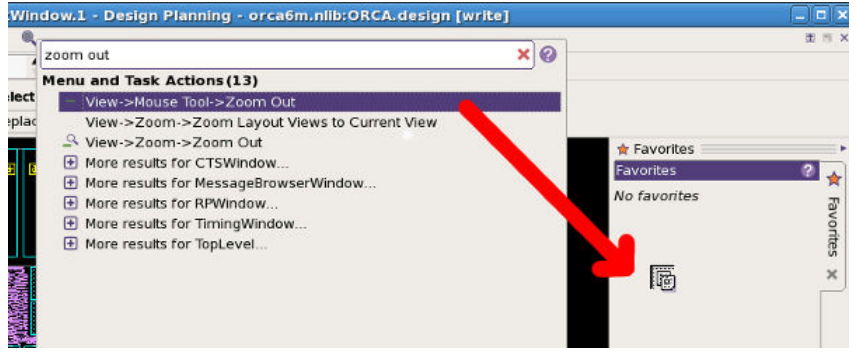
\includegraphics[width=0.92\textwidth]{gui-fig-197.png}
\caption{把按钮拖到 Favorites 调色板}
\label{fig:gui-197}
\end{figure}

% ============================================================
\section{用 Tcl 命令高亮对象}
\subsection*{Highlighting Objects With Tcl Commands}

用 Tcl 命令可以在 GUI 中高亮（highlight）对象，以不同颜色显示，便于识别。也可以定义要着色的对象集合（collection）。

\begin{itemize}
  \item 用三种不同颜色高亮 \cmd{NAND2*}、\cmd{NAND3*} 与 \cmd{NAND4*} 单元，见图~\ref{fig:gui-198}。
\end{itemize}

\begin{lstlisting}
gui_change_highlight -color yellow
   -collection [get_cells -hier -filter "ref_name=~NAND2*"]
gui_change_highlight -color red
   -collection [get_cells -hier -filter "ref_name=~NAND3*"]
gui_change_highlight -color light_blue
   -collection [get_cells -hier -filter "ref_name=~NAND4*"]
\end{lstlisting}

\begin{figure}[htbp]
\centering
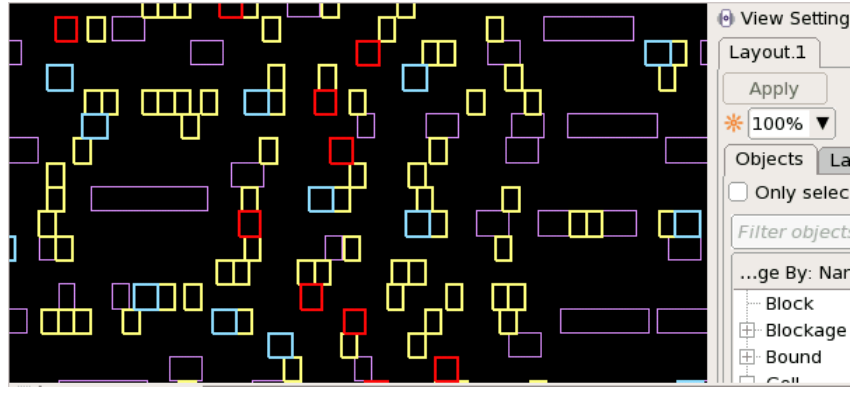
\includegraphics[width=0.92\textwidth]{gui-fig-198.png}
\caption{高亮的单元}
\label{fig:gui-198}
\end{figure}

\begin{itemize}
  \item 删除红色高亮。
\end{itemize}

\begin{lstlisting}
gui_change_highlight -color red -remove
\end{lstlisting}

\begin{itemize}
  \item 删除全部高亮。
\end{itemize}

\begin{lstlisting}
gui_change_highlight -all_colors -remove
\end{lstlisting}

% ============================================================
\section{创建标注}
\subsection*{Creating Annotations}

要向版图视图添加信息，可用标注创建直线、矩形、多边形和文字。标注不会保存到设计数据库，因此不具有持久性。用 \cmd{gui\_add\_annotation} 命令添加标注；用 \cmd{gui\_remove\_annotations} 命令删除标注。要创建持久标注，请使用 \cmd{create\_annotation\_shape} 命令。

\begin{seeAlsoBox}
详见第~\ref{chap:gui-anno}~章「创建持久标注」。
\end{seeAlsoBox}

下列示例创建不同类型的标注。最后一个示例删除全部标注。

\begin{itemize}
  \item 添加一条直线标注，见图~\ref{fig:gui-199}。
\end{itemize}

\begin{lstlisting}
gui_add_annotation -window Layout.1 -type line -color yellow \
   -width 4 {{67 2748} {636 2748}}
\end{lstlisting}

\begin{figure}[htbp]
\centering
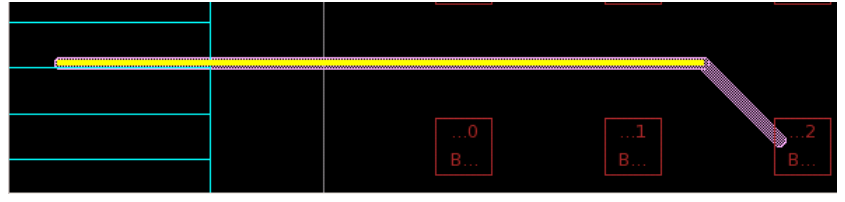
\includegraphics[width=0.92\textwidth]{gui-fig-199.png}
\caption{直线标注}
\label{fig:gui-199}
\end{figure}

\begin{itemize}
  \item 添加一条灰色直线，从单元 \cmd{pad\_iopad\_40} 的中心连到单元 \cmd{left\_15\_2} 的中心，并用十六进制值指定颜色，见图~\ref{fig:gui-200}。
\end{itemize}

\begin{lstlisting}
set cell1 [get_cells pad_iopad_40]
set cell2 [get_cells left_15_2]
gui_add_annotation -window Layout.1 -width 5 -color #999999 \
   -type line [list [list $cell1 center] [list $cell2 center]]
\end{lstlisting}

\begin{figure}[htbp]
\centering
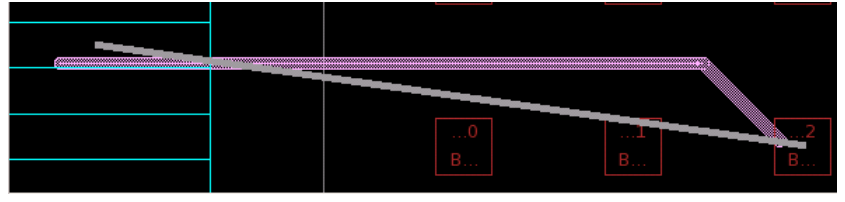
\includegraphics[width=0.92\textwidth]{gui-fig-200.png}
\caption{单元之间的直线标注}
\label{fig:gui-200}
\end{figure}

\begin{itemize}
  \item 添加一条矩形标注，见图~\ref{fig:gui-201}。
\end{itemize}

\begin{lstlisting}
gui_add_annotation -window Layout.1 -type rect -color red \
   -width 4 {{65 2700} {640 2800}}
\end{lstlisting}

\begin{figure}[htbp]
\centering
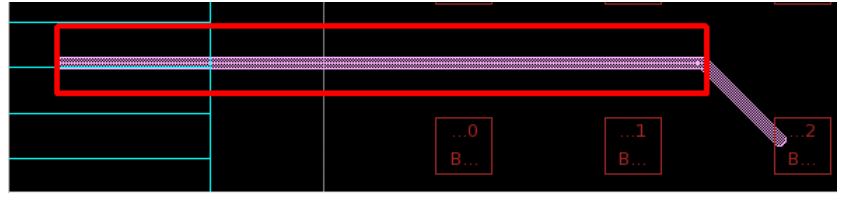
\includegraphics[width=0.92\textwidth]{gui-fig-201.png}
\caption{矩形标注}
\label{fig:gui-201}
\end{figure}

\begin{itemize}
  \item 添加一条文字标注。必须确保包围盒（bounding box）足够大，能够容纳文字。见图~\ref{fig:gui-202}。
\end{itemize}

\begin{lstlisting}
gui_add_annotation -window Layout.1 -type text -color white \
   -text "RDL Route" {{65 2715} {640 2815}}
\end{lstlisting}

\begin{figure}[htbp]
\centering
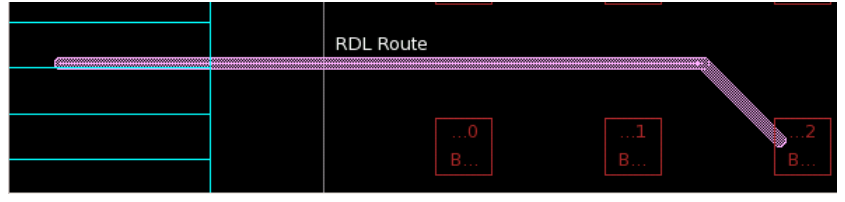
\includegraphics[width=0.92\textwidth]{gui-fig-202.png}
\caption{文字标注}
\label{fig:gui-202}
\end{figure}

\begin{itemize}
  \item 添加多条标注，并为每条标注附上信息提示（infotip），见图~\ref{fig:gui-203}。
\end{itemize}

\begin{lstlisting}
set net pad[40]
set shapes [get_shapes -q -of_objects $net]
foreach_in_collection shape $shapes {
  set len [get_attribute $shape length]
  gui_add_annotation -window Layout.1 -type line \
     -color yellow -width 4 \
     -info_tip "RDL Route $net\nLength = $len" \
     [get_attribute $shape points]
}
\end{lstlisting}

\begin{figure}[htbp]
\centering
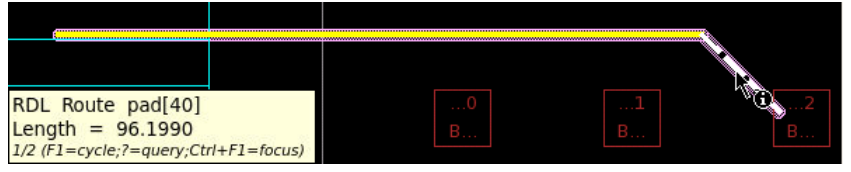
\includegraphics[width=0.92\textwidth]{gui-fig-203.png}
\caption{带信息提示的标注}
\label{fig:gui-203}
\end{figure}

\begin{itemize}
  \item 添加两个圆形标注，半径均为 100，见图~\ref{fig:gui-204}。
\end{itemize}

\begin{lstlisting}
gui_add_annotation -type circle -color yellow -width 2 \
   -radius 100 {{0 0}}
gui_add_annotation -type circle -color red \
   -width 2 {{200 0} {300 0}}
\end{lstlisting}

\begin{figure}[htbp]
\centering
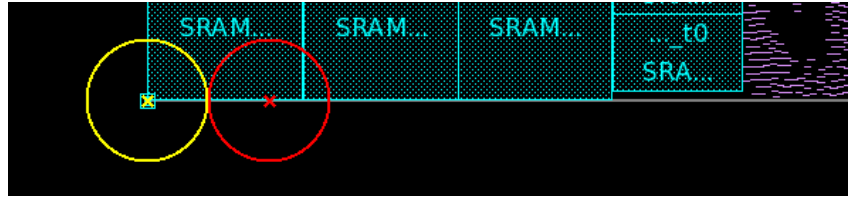
\includegraphics[width=0.92\textwidth]{gui-fig-204.png}
\caption{圆形标注}
\label{fig:gui-204}
\end{figure}

\begin{itemize}
  \item 创建两个圆形标尺（circular ruler），圆心分别为 (0, 0) 与 (400, 0)，见图~\ref{fig:gui-205}。
\end{itemize}

\begin{lstlisting}
gui_add_annotation -type circular_ruler \
   -color light_green {{0 0} {100 0}}
gui_add_annotation -type circular_ruler \
   -color light_purple {{400 0} {500 0} {700 0}}
\end{lstlisting}

可以再指定若干点，从而以同一圆心创建更多圆形标尺。用 \cmd{gui\_add\_annotation} 命令创建圆形标尺时，会忽略 \opt{-text}、\opt{-pattern}、\opt{-width} 和 \opt{-line\_style} 选项。

\begin{figure}[htbp]
\centering
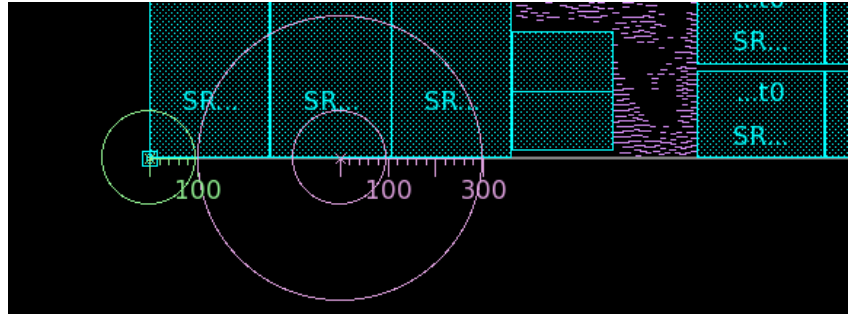
\includegraphics[width=0.92\textwidth]{gui-fig-205.png}
\caption{圆形标尺}
\label{fig:gui-205}
\end{figure}

\begin{itemize}
  \item 创建一条 45 度角的圆形标尺，见图~\ref{fig:gui-206}。
\end{itemize}

\begin{lstlisting}
gui_add_annotation -type circular_ruler -color light_purple \
   {{0 0} {70.171 70.711} {141.421 141.421}}
\end{lstlisting}

\begin{figure}[htbp]
\centering
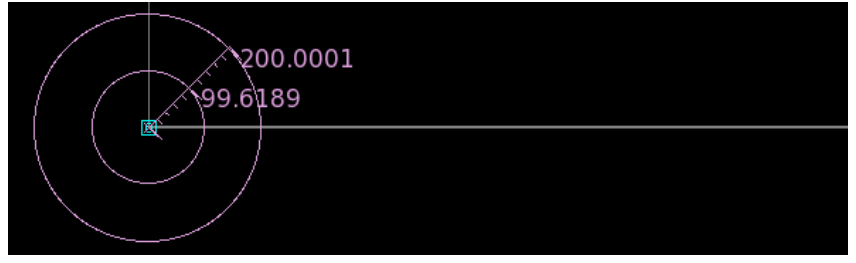
\includegraphics[width=0.92\textwidth]{gui-fig-206.png}
\caption{45 度圆形标尺}
\label{fig:gui-206}
\end{figure}

\begin{itemize}
  \item 从当前窗口删除全部标注。
\end{itemize}

\begin{lstlisting}
gui_remove_annotations \
   -window [gui_get_current_window -view -mru]
\end{lstlisting}

\begin{itemize}
  \item 从所有窗口删除全部标注。
\end{itemize}

\begin{lstlisting}
gui_remove_annotations [gui_get_annotations]
\end{lstlisting}

% ============================================================
\section{保存标注}
\subsection*{Saving Annotations}

要把 \cmd{gui\_add\_annotation} 命令创建的标注写到文件，使用 \cmd{gui\_write\_annotations} 命令。默认情况下，\cmd{gui\_write\_annotations} 写出全局标注（global annotation）。要写出当前全部版图标注，请带上参数 \cmd{[gui\_get\_annotations]}。

用下列选项控制 \cmd{gui\_write\_annotations} 命令的输出。
\begin{itemize}
  \item \opt{-file} \cmd{file\_name}：指定输出文件名。
  \item \opt{-append}：把输出追加到指定文件。默认情况下，若用 \opt{-file} 选项指定已存在的文件，命令会发出错误消息。
  \item \opt{-force}：覆盖指定的输出文件。
  \item \opt{-compress} \cmd{gzip}：用 gzip 压缩输出文件。
  \item \cmd{annotations}：指定要写入输出文件的标注。
\end{itemize}

下列示例创建两条标注：从 (0, 0) 到 (200, 200) 的直线标注，以及位于 (0, 0) 的圆形标注。

\begin{noteBox}
第一条标注使用 \opt{-window} 选项指定窗口，第二条标注不带该选项。
\end{noteBox}

\begin{lstlisting}
gui_add_annotation -window Layout.1 -type line -color yellow \
   -width 4 {{0 0} {200 200}}
gui_add_annotation -type circular_ruler \
   -color red {{0 0} {100 0}}
\end{lstlisting}

这些命令在版图中创建下列标注，见图~\ref{fig:gui-207}。

\begin{figure}[htbp]
\centering
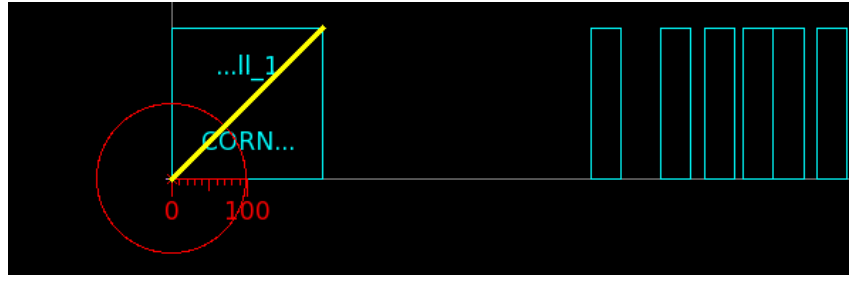
\includegraphics[width=0.92\textwidth]{gui-fig-207.png}
\caption{直线与圆形标注}
\label{fig:gui-207}
\end{figure}

\cmd{gui\_write\_annotations} \opt{-file} \cmd{file\_name} \cmd{[gui\_get\_annotations]} 命令写出全部全局标注和特定于窗口的标注。
\begin{lstlisting}
icc2_shell> gui_write_annotations \
   -file all_gui_annotations.tcl [gui_get_annotations]
icc2_shell> sh cat all_gui_annotations.tcl
...
set Layout_1 Layout.1
gui_add_annotation -window $Layout_1 -group global -type polyline \
   -color yellow -pattern NoBrush -line_style SolidLine \
   -width 4 {{0.000 0.000} {200.000 200.000}}
gui_add_annotation -window global -group global \
   -type circular_ruler -color red -pattern NoBrush \
   -line_style SolidLine -width 1 {{0.000 0.000} {100.000 0.000}}
\end{lstlisting}

\cmd{gui\_write\_annotations} \opt{-file} \cmd{file\_name} 命令只写出全局标注（未使用 \opt{-window} 选项指定的标注）。
\begin{lstlisting}
icc2_shell> gui_write_annotations -file global_gui_annotations.tcl
icc2_shell> sh cat global_gui_annotations.tcl
...
gui_add_annotation -window global -group global \
   -type circular_ruler -color red -pattern NoBrush \
   -line_style SolidLine \
   -width 1 {{0.000 0.000} {100.000 0.000}}
\end{lstlisting}

% ============================================================
\section{创建新的视觉模式}
\subsection*{Creating New Visual Modes}

视觉模式（visual mode）以彩色叠层（overlay）高亮设计信息。可用视觉模式高亮设计中的不同元素，并把这些元素组织到各个箱（bin）中。\cmd{gui\_create\_vm} 与 \cmd{gui\_create\_vmbucket} 命令用于定义新的视觉模式、创建单独的箱，并把一个集合关联到每个箱。

下列示例创建一个新的视觉模式，按设计层次（design hierarchy）的不同部分为宏单元（macro）着色。\cmd{gui\_create\_vm} 命令创建名为 \textbf{Macros} 的新视觉模式。启动 \textbf{Macros} 视觉模式后，单击 \textbf{Reload} 按钮时会调用 \cmd{reload\_macros\_vm} 过程（procedure）。\cmd{gui\_create\_vmbucket} 命令把该视觉模式中的各个箱指定到具体集合。\cmd{gui\_show\_map} 命令打开视觉模式调色板（Visual Mode palette），并显示新的 \textbf{Macros} 视觉模式。工具显示出 Visual Mode 调色板后，单击 \textbf{Reload} 按钮即可为宏单元着色。

\begin{seeAlsoBox}
关于 Visual Mode 调色板的更多信息，见第~\ref{chap:gui-map}~章「视觉模式概述」。
\end{seeAlsoBox}

\begin{lstlisting}
gui_create_vm -name Macros -update_cmd reload_macros_vm
proc reload_macros_vm {args} {
  set vm Macros
  gui_remove_vmbucket -vmname $vm -all
  set collection_1 [get_cells -physical_context \
     -filter "is_hard_macro && full_name=~I_CLOCK_GEN/*"]
  set collection_2 [get_cells -physical_context \
     -filter "is_hard_macro && full_name=~I_ORCA_TOP/I_PCI_TOP/*"]
  set collection_3 [get_cells -physical_context \
     -filter "is_hard_macro && full_name=~I_ORCA_TOP/I_CONTEXT_MEM/*"]
  set collection_4 [get_cells -physical_context \
     -filter "is_hard_macro && full_name=~I_ORCA_TOP/I_RISC_CORE/*"]

  gui_create_vmbucket -vmname $vm -name clock_gen \
     -title {clock_gen} -color red -collection $collection_1
  gui_create_vmbucket -vmname $vm -name pci_top \
     -title {pci_top} -color green -collection $collection_2
  gui_create_vmbucket -vmname $vm -name context_mem \
     -title {context_mem} -color blue -collection $collection_3
  gui_create_vmbucket -vmname $vm -name risc_core \
     -title {risc_core} -color yellow -collection $collection_4
}
gui_show_map -map Macros -show true
\end{lstlisting}

见图~\ref{fig:gui-208}。

\begin{figure}[htbp]
\centering
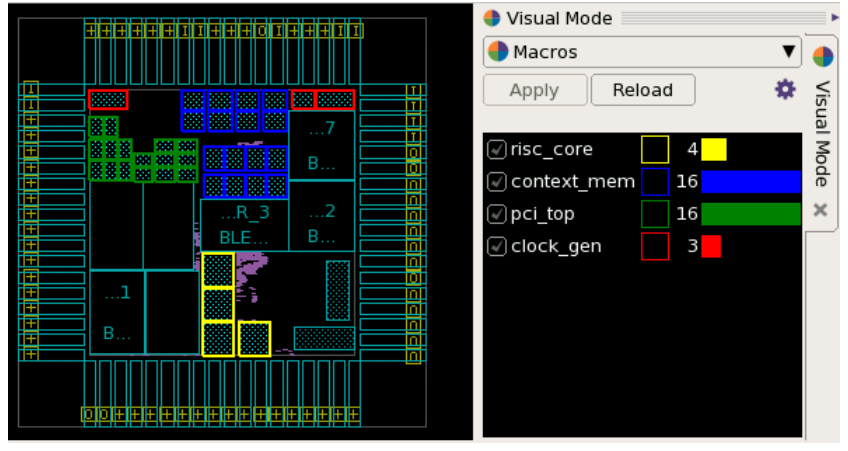
\includegraphics[width=0.92\textwidth]{gui-fig-208.png}
\caption{自定义视觉模式}
\label{fig:gui-208}
\end{figure}
